\documentclass[tikz, border=3.14pt]{standalone}    
\usepackage{pgfplots}    
\pgfplotsset{compat=1.17}    
\usepackage{darkmode}    
\enabledarkmode    
    
\pgfplotsset{    
  colormap={mycolormap}{    
    rgb(0.0000)=(0.6667,0.2941,0.5255)  % 170,75,134    
    rgb(0.0625)=(0.5765,0.3608,0.4627)  % 147,92,118    
    rgb(0.1250)=(0.5529,0.3765,0.4471)  % 141,96,114    
    rgb(0.1875)=(0.5098,0.4078,0.4157)  % 130,104,106    
    rgb(0.2500)=(0.4902,0.4235,0.4000)  % 125,108,102    
    rgb(0.3125)=(0.4392,0.4630,0.3647)  % 112,118,93    
    rgb(0.3750)=(0.4000,0.4902,0.3373)  % 102,125,86    
    rgb(0.4375)=(0.3647,0.5176,0.3098)  % 93,132,79    
    rgb(0.5000)=(0.3294,0.5412,0.2863)  % 84,138,73    
    rgb(0.5625)=(0.3020,0.5647,0.3412)  % 77,144,87    
    rgb(0.6250)=(0.2745,0.5882,0.4039)  % 70,150,103    
    rgb(0.6875)=(0.2392,0.6196,0.4824)  % 61,158,123    
    rgb(0.7500)=(0.1922,0.6627,0.5843)  % 49,169,149    
    rgb(0.8125)=(0.1686,0.6824,0.6314)  % 43,174,161    
    rgb(0.8750)=(0.1216,0.7216,0.7333)  % 31,184,187    
    rgb(0.9375)=(0.0863,0.7529,0.8078)  % 22,192,206    
    rgb(1.0000)=(0.0000,0.8314,1.0000)  % 0,212,255    
  },    
  colormap={gray}{    
    rgb255(0)=(100,100,100),    
    rgb255(1)=(100,100,100)    
  }    
}    
    
\definecolor{varred}{RGB}{221,123,102}  
\definecolor{varcyan}{RGB}{82,139,128}  
\definecolor{varblue}{RGB}{96,159,179}  
\definecolor{varyellow}{RGB}{225,224,91}  
\definecolor{vargreen}{RGB}{135,174,117}  
\definecolor{varpurple}{RGB}{235,89,185}  
    
\begin{document}    
    
\pagecolor{black}    
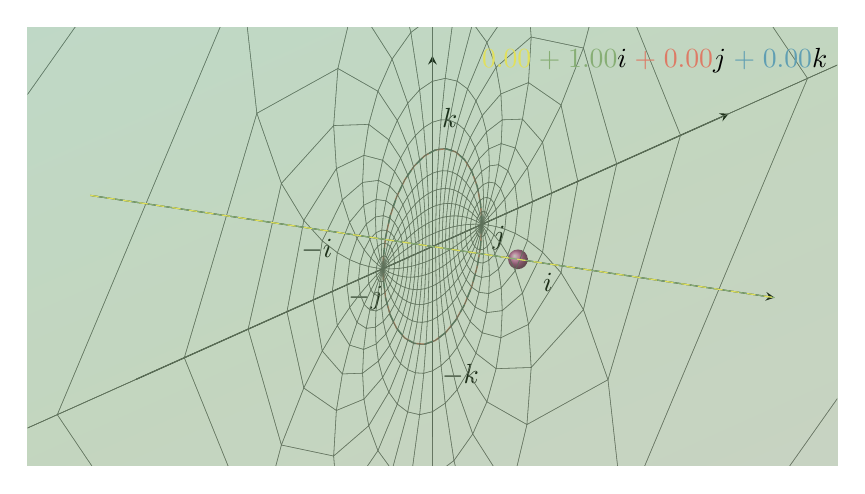
\begin{tikzpicture}    
    \begin{axis}[    
        view={30}{15},    
        axis lines=center,    
        xmin=-4, xmax=4,    
        ymin=-6, ymax=6,    
        zmin=-2, zmax=2,    
        axis equal image,    
        clip=false,    
        xtick=\empty,    
        ytick=\empty,    
        ztick=\empty,    
        scale=3    
    ]    
        \clip (-3,-3,-2) rectangle (3,3,2);
        \shade[ball color=varpurple] (axis cs:1,0,0) circle (0.125cm);    
        \node[below] at (axis cs:1.35,0,0) {$i$};    
        \node[below] at (axis cs:-1.35,0,0) {$-i$};    
        \node[below] at (axis cs:0,1.35,0) {$j$};    
        \node[below] at (axis cs:0,-1.35,0) {$-j$};    
        \node[right] at (axis cs:0,0,1.35) {$k$};    
        \node[right] at (axis cs:0,0,-1.35) {$-k$};    
          
        \draw [  
            varred,  
            domain=0:360,  
            samples=30,  
            variable=\theta,  
            line width=0.5pt,  
        ] plot(  
            0,  
            {cos(\theta)},  
            {sin(\theta)}  
        );  
        \draw [  
            varcyan,  
            dashed,  
            domain=0:360,  
            samples=30,  
            variable=\theta,  
            line width=0.5pt,  
        ] plot(  
            0,  
            {cos(\theta)},  
            {sin(\theta)}  
        );  
    
        \addplot3 [    
            domain=0:180,    
            domain y=0:360,    
            samples=25,    
            samples y=25,    
            mesh,    
            colormap name=gray,    
            shader=interp,    
            line width=0.2pt,    
            z buffer=sort,    
            variable=\t,    
            variable y=\p,    
            opacity=0.75    
        ]    
        (    
            0,  
            {-cos(\t)/(1 + sin(\t)*cos(\p))},  
            {sin(\t)*sin(\p)/(1 + sin(\t)*cos(\p))}  
        );    
        \addplot3 [    
            domain=0:180,    
            domain y=0:360,    
            samples=50,    
            samples y=50,    
            surf,    
            colormap name=mycolormap,    
            shader=interp,    
            line width=0.2pt,    
            z buffer=sort,    
            variable=\t,    
            variable y=\p,    
            opacity=0.35    
        ]    
        (    
            0,  
            {-cos(\t)/(1 + sin(\t)*cos(\p))},  
            {sin(\t)*sin(\p)/(1 + sin(\t)*cos(\p))}  
        );  
          
        \draw[vargreen] (axis cs:-4,0,0) -- (axis cs:4,0,0);
        \draw[varyellow, dashed] (axis cs:-4,0,0) -- (axis cs:4,0,0);  
        \node[left] at (axis cs:3,3,1.65) {${\color{varyellow} 0.00} {\color{vargreen} \;+\; 1.00}i{\color{varred} \;+\; 0.00}j{\color{varblue} \;+\; 0.00}k$};    
    \end{axis}    
\end{tikzpicture}    
\end{document}
